%\documentclass[12pt]{report}	
%\input{Formatting_TEMPL8}
%
%% Make start at chapter 2
%\setcounter{chapter}{0}
%\begin{document}
	
% ===================
	\chapter{Introduction}
	\cite{pahl2016interference} 
	\lipsum[1] \cite{stankevivcius2014electromagnetic}
	
	
	\section{Background of the Study}
	\lipsum[2-3]
	
	\begin{figure}[htbp]
		\begin{adjustwidth}{1.25cm}{0pt}
			\centering
			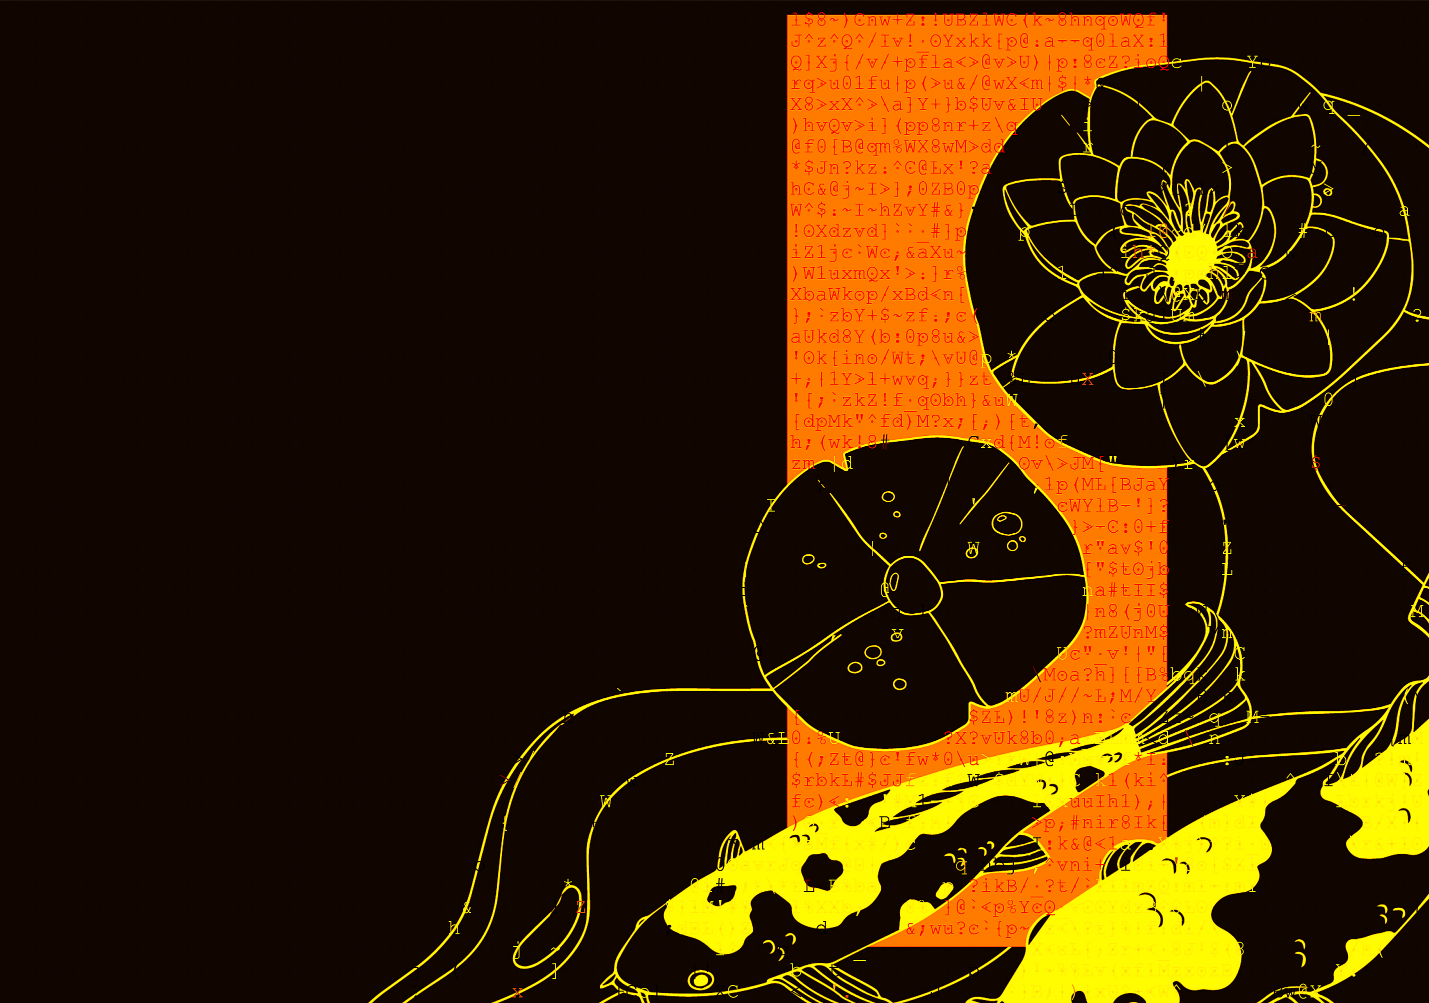
\includegraphics[scale=0.35]{samplefig}
			\caption{Basic elements of a communication system \cite{pahl2016interference}}
			\label{fig:samplefig}
		\end{adjustwidth}
	\end{figure}
	
	Figure~\ref{fig:samplefig} \lipsum[4] 
	
	\subsection{Statement of the Problem}
	\lipsum[1]
	
	\begin{figure}[htbp]
		\begin{adjustwidth}{1.25cm}{0pt}
			\centering
			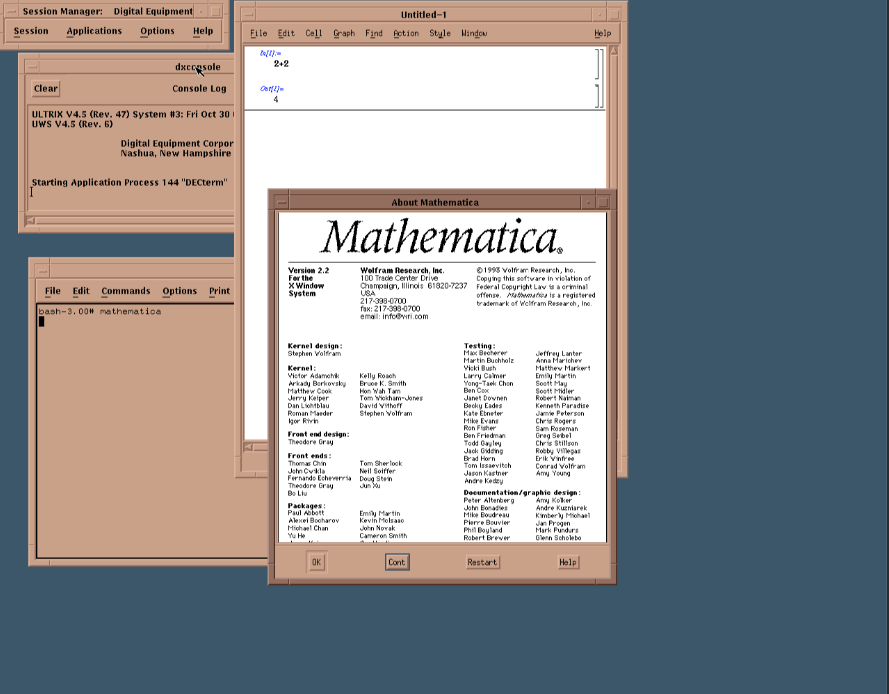
\includegraphics[scale=0.5]{nest/samplefig2.png}
			\caption{Basic elements of a communication system }
			\label{fig:samplefig2}
		\end{adjustwidth}
	\end{figure}
	\cite{pahl2016interference}
	 Figure~\ref{fig:samplefig2} \lipsum[2]
	
%	
%	\bibliographystyle{IEEEtran}
%	\bibliography{references_TEMPL8}
%\end{document}
